%Template by Mark Jervelund - 2015 - mjerv15@student.sdu.dk

\documentclass[a4paper,10pt,titlepage]{report}

\usepackage[utf8]{inputenc}
\usepackage[T1]{fontenc}
\usepackage[english]{babel}
\usepackage{amssymb}
\usepackage{amsmath}
\usepackage{amsthm}
\usepackage{graphicx}
\usepackage{fancyhdr}
\usepackage{lastpage}
\usepackage{listings}
\usepackage{algorithm}
\usepackage{algpseudocode}
\usepackage[document]{ragged2e}
\usepackage[margin=1in]{geometry}
\usepackage{color}
\usepackage{datenumber}
\usepackage{venndiagram}
\usepackage{chngcntr}
\setdatetoday
\addtocounter{datenumber}{0} %date for dilierry standard is today
\setdatebynumber{\thedatenumber}
\date{}
\setcounter{secnumdepth}{0}
\pagestyle{fancy}
\fancyhf{}

\newcommand{\Z}{\mathbb{Z}}
\lhead{Computer Architecture (DM548))}
\rhead{Mark Jervelund (Mjerv15)}
\rfoot{Page  \thepage \, of \pageref{LastPage}}
\counterwithin*{equation}{section}

\begin{document}
\renewcommand{\thepage}{\roman{page}}% Roman numerals for page counter
\tableofcontents
\newpage
\setcounter{page}{1}
\renewcommand{\thepage}{\arabic{page}}
\section{Course description}
To describe the services an operating system provides to
users, processes, and other systems\\
To discuss the various ways of structuring an operating
system\\
To explain how operating systems are installed and
customized and how they boot\\
\newpage
\section{Question 1 - Operating System Structures - ch 2}
%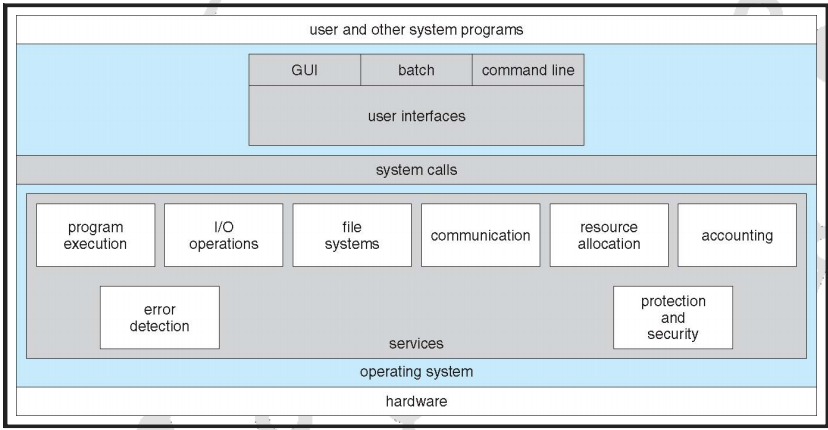
\includegraphics[scale=0.5]{Picture1.png}
User interfaces = Command-Line (CLI), Graphics User Interface (GUI), Batch \\


\subsection{Keywords}
1.) Short introduction \\
\hspace{10mm}explain the 3 types of interfaces. GUI, CLI, and batch\\
\hspace{15mm}Explain pros and cons\\
\hspace{20mm}CLI - Requires more knowlage about how it works. \\
\hspace{20mm}GUI - More intuative and easier to use \\
\vspace{5mm}


2.)

How you communicate between OS and programs,\\
\hspace{10mm}System calls - How do you call them, how to use them. parameters etc. \\
\hspace{15mm} Check file with the list of system calls \\
\hspace{15mm} Find the file corresponding to the system call.\\
\hspace{15mm} puts the parameters\\
\hspace{20mm} using registers\\
\hspace{20mm} stores in block and address of block is passed to the function as a parameters\\
\hspace{20mm} places or pushed on the stack and POPed by the operating system.\\
\vspace{5mm}


3*)
Process communications \\
\hspace{10mm}Message parsing and shared memory \\ 
\hspace{15mm} pro/cons \\
\hspace{10mm} shared memory, uses less space as memory is only copied if it gets changed.\\
\hspace{10mm} Message parsing\\
\hspace{15mm} Either directly between two processes via mailbox handled by the os \\
\vspace{5mm}


4*) 
OS structure \\ 

\hspace{10mm}	Simple structure \\
\hspace{15mm}    	There is no control, applications can talk directly to hardware and the kernel.\\


\hspace{10mm}    Layered \\
\hspace{15mm}    	There are multiple layers,the user can only talk to the the applications,the applications can only talk to the operating system API, and only the operating system can call to the kernel \\
\hspace{15mm}        User->Application->OS->Hardware \\

\hspace{10mm}	Micro-kernel\\
\hspace{15mm}		Move as much as the kernel as you can into user-space. User mode applications can communicate via the kernel.
    
\hspace{10mm}   Modules \\
\hspace{15mm}		Indivisdual modules that can be loaded and unloaded into the kernel, so provide some kind of use.
                
\hspace{10mm}    Hybrid-systems \\
\hspace{15mm} Most modern operating systems are not one pure model, 



\vspace{5mm}


5) Debugging\\
\hspace{10mm}What can we do when something goes wrong? \\
\hspace{15mm}	Log files, data dumps, tracing tools. Windows task-manager essential, Linux has the top/htop command \\

\vspace{5mm}


6) Boot-loaders, How does the os know where to find the boot-loader, kernel, etc. \\
\hspace{10mm} Multiple stages, Bios loads a 512(less due to constraints)boot loader into memory from the master boot record on a disk and jumps to it. this then either loads a secondary bootloader, or the kernel.




\newpage
\subsection{Questions from lecture}
What is a system call.\\
\hspace{10mm} Programming interface to the services provided by the operating system \\ \vspace{5mm}


What groups of system calls are there. \\
\hspace{10mm}File manipulation, process control, security and protection, communication, I/O device manipulation \& information management\\ \vspace{5mm}


why would you use a system call API.\\
\hspace{10mm}Ease of use, Reduce failure, reuseability/portability \\ \vspace{5mm}


What ways are there to pass parameters to the OS.\\
\hspace{10mm} Stack + reference, register, memory -> send reference \\  \vspace{5mm}


How can an operating system be structured(architecture wise)\\
\hspace{10mm} Layered structure, module based, micro-kernel \& hybrid systems\\ \vspace{5mm} 


what code is first read when you turn on your computer\\
\hspace{10mm}Bootstrap code located in EPROM \\ \vspace{5mm}





\newpage
\section{Question 2 - Process Concept and Multi threaded Programming - ch 3 \& 4}
\subsection{Keywords}
1) Introduction - Process control block. \\ Diagram on slide 3.7\\
\hspace{10mm}	What is a process. \\
\hspace{10mm}	Process control block. \\
\hspace{15mm}	State \\
\hspace{15mm}	Process number \\
\hspace{15mm}	Program counter \\
\hspace{15mm} 	Registers \\
\hspace{15mm}	Memory limits \\
\hspace{15mm} 	Files descriptors (active files ) \\
\hspace{15mm} 	.... \\
\vspace{5mm}


2) Process scheduling - \\
\hspace{10mm}	CPU \& I/O burst \\
\hspace{10mm}	Short, medium \& long schedulers.\\
\hspace{15mm}   Short - ready, running and waiting. \\
\hspace{15mm}	Medium - Swaps Out to disk. \\
\hspace{15mm}	Long - Loads jobs into the new queue from a work queue. \\
\vspace{5mm}


3) Context switch.\\
\hspace{10mm} Saves current state of the process and stores it, when the process waits for I/O.\\
\vspace{5mm}



4) Interprocess communication - \\
\hspace{10mm}	Message parsing \\
\hspace{15mm}  	The processes can communicate with each other without resorting to shared variables	\\
\hspace{15mm} 	This is done using by using a IPC facility that has two operations. a send and a receive operation.\\
\hspace{15mm} 	If eg. P and Q wish to communicate they'll need to first establish a link between them, and then exchange the message via send/receive. \\
\hspace{15mm} Direct and indirect(mailbox with id) \\


\hspace{10mm}	Shared memory \\
\hspace{15mm}	Fixed shared memory segment \\
\hspace{15mm}	The processes have to check if the memory changed. \\
\vspace{5mm}

5) Communication-Client/server\\

\hspace{10mm}	RPC (Remote Procedure Call )\\
\hspace{15mm}	Abstract procedure calls on networked systems \\
\hspace{10mm}	Socket \\
\hspace{15mm}	pair of sockets using TCP/UDP - Ip:port \\
\hspace{10mm}	Pipes\\
\hspace{15mm}   Unamed pipes - Unidirectional, and require parent child relation\\
\hspace{15mm} 	Named pipes - bidirectional, and can be used by multiple processes. \\
\vspace{5mm}




6) Multitreading models\\
\hspace{10mm} Many to one \\
\hspace{10mm} One to One \\
\hspace{10mm} Many to Many \\	
\hspace{10mm} Hybrid - 2 level model \\
\vspace{5mm}

7) Multicore programming \\
\hspace{10mm} Amdahl Law - S is serial portion and n is processing cores.
\begin{equation}
speedup = \frac{1}{S+\frac{1-S}{N}}
\end{equation}
\vspace{5mm}

8) Concurrency /parallel - \\
\hspace{10mm} Whats the difference\\
\hspace{15mm} Concurrency \\
\hspace{20mm} One program using multiple threads doing different things. eg, consumer/producer \\
\hspace{15mm} parallel \\
\hspace{20mm} A program using multiple threads to do the same work. \\
\vspace{5mm}

9) Thread libraries \\
\hspace{10mm} POSIX \\
\hspace{10mm} Pthread \\
\hspace{10mm} javathread \\
\hspace{10mm} Winthread(win32) \\
\vspace{5mm}

10) Implicit Threading \\
\hspace{10mm} Thread pools \\
\hspace{10mm} OpenMP - Compiler finds code that can be run in parallel and compiles it so it is. \\
\hspace{10mm} Grand Central dispatch - Allows identification of parallel sections, manages most of the details. \\
\hspace{15mm} two types of queues, serial where its FIFO and concurrent. removed in FIFO but multiple items can be removed at the same time. \\
\vspace{5mm}

11) Threading Issues \\
\hspace{10mm} Signal handling \\
\hspace{10mm} Thread Cancellation - When should a thread be terminated \\
\hspace{10mm} Thread-Local Storage - Each thread had its own copy of the data(waste of space)\\
\hspace{10mm} Scheduler activations \\
\vspace{5mm}





\newpage
\subsection{Questions from lecture}
What state can a process by in?\\
\hspace{10mm}New.\\
\hspace{10mm}Ready.\\
\hspace{10mm}running.\\
\hspace{10mm}waiting.\\
\hspace{10mm}terminated.\\
\vspace{5mm}




What is a process control block?\\
\hspace{10mm}A block where the OS store information about a program.\\ 
\hspace{10mm}Used for content switching and stores the following information:\\
\hspace{20mm}Process state\\
\hspace{20mm}Process number\\
\hspace{20mm}Process counter\\
\hspace{20mm}Registers\\
\hspace{20mm}Memory limits\\
\hspace{20mm}List of open files\\


\vspace{5mm}
Describe ways to do IPC\\
\hspace{10mm}Message parsing and memory shearing. \\




\vspace{5mm}
What is the difference between a process and a thread\\
\hspace{10mm}A process is a thing we need to execute, and thread is a subtask of a process.\\


\vspace{5mm}
What advantages is there when using threads?\\
\hspace{10mm}Threading lets you work on multiple cores at the same time, therefor letting you run a job faster.\\


\vspace{5mm}
Difference between parallelism and concurrency?\\

\hspace{10mm}	Parallelism - same task spread on multiple threads\\
\hspace{10mm}	Concurrency - program running with multiple threads\\
\hspace{10mm}  	We can have Concurrency without Parallelism but not the other way around\\



\vspace{5mm}
What are the most common API's for user level threads\\
\hspace{10mm} Boost (maybe builds on pthread) \\
\hspace{10mm} Pthread \\
\hspace{10mm} Java thread \\
\hspace{10mm} Winthread \\
\vspace{5mm}



What are the implicit threading methods.\\
\hspace{10mm} Thead pools \\
\hspace{10mm} Openmp \\
\hspace{10mm} Grand Central Dispatch \\

\newpage

\section{Question 3 - Process Scheduling - ch 5}
Scheduling types\\
FCFS - unstable wait time.\\
Shortest job first. optimal. gives minium wait time, but only usable for long time sheduling.\\
\vspace{5mm}

\subsection{Keywords}
1. Introduktion\\
\hspace{10mm}what is CPU bound\\
\hspace{10mm}what is I/O bound\\
\hspace{10mm}explain as shortterm, medium term, and long term\\
2. Criterias\\
\hspace{10mm}What do we want to take a look at as I/O bound, like what can we do to get a better CPU Util\\
3. Algorithmer \\ 
\hspace{10mm}Explain FCFS, SJF, etc.\\
\hspace{10mm} Schedulers.\\
\hspace{15mm} First come first service\\
\hspace{15mm} Shortest job first \\
\hspace{15mm} Shortest time remaining first \\
\hspace{15mm} Round robin\\
\hspace{15mm}give each process the same amount of time and loop over them until they're done. circular queue\\
\hspace{10mm}starvation etc. \\
4. Multi processer scheduling.\\
\hspace{10mm}Single queue, queue per core, shared queues\\
5. Realtime schduling\\

6. Examples\\
\newpage
\subsection{Questions from lecture}
1. When is it Relevent for the scheduler to take  decision.\\
\hspace{10mm}When a new process queued, and a new processes is started.\\
\hspace{10mm}4 cases\\
\hspace{20mm}when a process running state to waiting.\\
\hspace{20mm}when a process terminates.\\
\hspace{20mm}When a process is queued\\
\hspace{20mm}When a process goes from waiting to ready\\

\vspace{5mm}

What is dispatch latency.\\
\hspace{10mm} time it takes for a interupting process to become active \\
\hspace{10mm} move memory and registers from the running task, move new tasks there and start it \\
\vspace{5mm}

What scheduling ctiteria can we use.\\
\hspace{10mm} maximize CPU util, low latency for take critical jobs jobs.\\
\hspace{10mm} runtime, priority, CPU bound, I/p bound \\
\vspace{5mm}

Describe the scheduling algortirhms: FCFS, SJF, Shortest remaining time fist, RR.\\
\hspace{10mm} First come first servce\\
\hspace{10mm} Shortest job first \\
\hspace{10mm} Shortest time remaining first \\
\hspace{10mm} Round robin\\
\hspace{10mm}give each process the same amount of time and loop over them until they're done. circular queue\\
\vspace{5mm}


Describe priority schduling and aging\\
\hspace{10mm} The longer it has been in the queue the higher the priority the job has\\
\vspace{5mm}

What is the difference betweeen asymmetric and symmetric multiprocessing\\
\hspace{10mm} Asymmmetric means tasks wont wait for other things \\
\hspace{10mm} Not all processes has the some capapicities\\
\hspace{10mm} All the kernals can do the same.\\ 
\vspace{5mm}

What is a memory stall\\
\hspace{10mm} Waiting for memory ? \\
\vspace{5mm}



What is the difference between soft and hard real-time systems.\\
\hspace{10mm} Soft -  Don't time life critital systems while hard real time systems have.\\
\vspace{5mm}




Describe rate montonic scheduling and earlist deadline scheduling\\
\hspace{10mm} rate montonic scheduling - Schedule jobs in intervals, like a, b, c.\\
\hspace{10mm} earliest deadline scheduling - Schedule the process with the first deadline first.\\
\vspace{5mm}



\newpage
\section{Question 4 - Synchronization - ch 6}


\subsection{Keywords}
1. Introduction\\

2. Critital section\\
\hspace{10mm}What is it?\\
\hspace{10mm}- The 3 requirements: mutual exclusion, progress, bounded waiting (Software
Solution) \\
\hspace{10mm}- Peterson's solution as example in book, but not too useful to cover \\
\vspace{5mm}



3. software solution to critical section\\
\vspace{5mm}



4. hardware solutions to critical section\\
\hspace{10mm} Why is hardware a better solution than software? \\
 	 	\hspace{10mm} 'test\_and\_set()' and 'compare\_and\_swap() \\
\vspace{5mm}


5. mutex lock\\
\hspace{10mm} Simplest \\
\hspace{10mm} Check a variable if we can enter section \\
\hspace{10mm} Setting/checking variables are NOT atomic actions so we need to use hardware help \\
\vspace{5mm}


6. semaphore lock\\
\hspace{10mm} More complex solution \\
\hspace{10mm} Allows for more customization \\
\hspace{10mm} Such as a MAX of processes at once \\
\vspace{5mm}


7. monitors\\
\hspace{10mm}  A lock that can release its locks again if all locks needed can't be acquired, this can be used to solve the dining philosophers problem. \\

\vspace{5mm}
8. spinlock\\
\hspace{10mm}  When do we want to use spin lock, and when do we use Mutex locks instead \\
\vspace{5mm}



9. examples\
\vspace{5mm}


10. alternative solution\\
\hspace{10mm} Usage of library such as OpenMP, which us define pragmas instead and functional
programming languages

\newpage
\subsection{Questions from lecture}

Describe the terms "race condition" and "Critical section"\\

\hspace{10mm} When two proceses want to access a shared resource. that may be unstable if its done in a \\ \hspace{10mm} non-locked way\\
\hspace{10mm} Race condition is when multiple processes/threads are competing about the same resources and \\ \hspace{10mm}  a undesired output may happen. \\
\hspace{10mm}  Critical section is a section of code that sensitive to race conditions.\\
\vspace{5mm}





What should a solution to the critical section satisfy \\
\hspace{10mm}  Mutual exclution, progress, and \\
\hspace{10mm}  that only one thread can be active in the critical section at the time. \\
\vspace{5mm}



What is preemptive vs. non preemptive \\

\hspace{10mm}  preemptive is the act is  temporarily interrupting a process\\

\hspace{10mm}  non-preemptive -  When a process enters the state of running, the state of that process is not \\ \hspace{10mm} deleted from the scheduler until it finishes its service time.\\
\vspace{5mm}


Describe "test and set" and "compare and swap". \\

\hspace{10mm}  Two different ways of implementing a mutex lock, that are garenttted to be excuted in an atomic \\ \hspace{10mm} way.\\

\hspace{10mm} Test and set - \\

\hspace{10mm}  Compare and swap can only be used by one function, its checks for a codition and sets swaps \\ \hspace{10mm}  two value if the condition is met.\\ 
\vspace{5mm}



What is a mutex and a semaphore \\

\hspace{10mm}  a Mutex lock is a lock where only the process holding the lock is allowed to perform actions in \\ \hspace{10mm}  	the locked section. \\
\hspace{10mm}  A mutex contains a boolean and is acquired and released.\\


\hspace{10mm}  A binary semaphore is the same as a mutex. \\

\hspace{10mm}  a counting semaphore is when the lock uses a counter if multiple processes can be active within \\
\hspace{10mm}  the lock. \\

\vspace{5mm}



Describe some classic problems of synchronization. \\

\hspace{10mm}  Readers writers problems.\\
\hspace{10mm} dining philosopher problem. \\
\vspace{5mm}




What is a monitor \\
\hspace{10mm}  We can put functions into the monitor and only one process can be active within the monitor \\
\hspace{10mm} at the time, else the process will have to wait in the queue.






\

\newpage
\section{Question 5 - Deadlocks - ch 7}
\subsection{Keywords}
1. Introduction\\
\hspace{10mm} What is a deadlock\\
\hspace{10mm} 4 conditions \\
\hspace{20mm} mutual exclusion, hold and wait, circular wait, and no pre-emption \\
\hspace{20mm} Show a small example, resource graph \\
\vspace{5mm}

2.  How to handle a deadlock \\
\hspace{10mm} Prevent and avoid \\
\hspace{10mm} recover \\
\hspace{15mm} Start killing tasks that are in the deadlock until its resolved \\
\hspace{10mm} Ignore \\
\hspace{15mm} Let the user handle it \\
\vspace{5mm}

3. How to avoid a deadlock \\
\hspace{10mm} How to avoid the 4 conditions \\
\hspace{15mm} If we can change one we can avoid \\
\vspace{5mm}

4. avoiding a deadlock \\
\hspace{10mm} bankers algorithm \\
\hspace{10mm} resources graphs \\
\hspace{10mm} what is the criteria for that they are in safe and unsafe states \\
\vspace{5mm}


5. Deadlock detection  \\
\hspace{10mm} resources graph detection \\
\vspace{5mm}



6. why do we want to avoid deadlocks\\
\hspace{10mm} give examples on when to avoid deadlocks.
\vspace{5mm}

7. Recover \\
\hspace{10mm} Show some algorithms on how to avoid a deadlock \\
\vspace{5mm}


8. Examples \\
\newpage


\subsection{Notes}

\subsubsection{Objectives}
To develop a description of deadlocks, which prevent sets of concurrent
processes from completing their tasks\\
To present a number of different methods for preventing or avoiding
deadlocks in a computer system\\
\subsubsection{What is a deadlock}
4 things have to hold for a deadlock to happen, these are Mutual exclusion
Hold and wait
No preemption
Circular wait
\\
Mutual exclusion\\
\hspace{10mm} Only one process at a time can use a resource\\
Hold and wait\\
\hspace{10mm} A process holding at least one resource is waiting to acquire additional
resources held by other processes \\
No preemption\\
\hspace{10mm} A resource can be released only voluntarily by the process holding it, after
that process has completed its task \\ 
Circular wait\\
\hspace{10mm} There exists a set {P0 , P1 , … , Pn } of waiting processes such that P0 is waiting
for a resource \\
\hspace{10mm} that is held by P1 , P1 is waiting for a resource that is held by
P2 , … , Pn–1 is waiting for a \\
\hspace{10mm}resource that is held by Pn, and Pn is waiting for a
resource that is held by P0. \\
\vspace{2mm} 
\hspace{10mm}We have a circle of tasks waiting for each other.
\\
\subsubsection{How can a deadlock be detected}

\subsubsection{Graph detection}
Deadlocks can be detected by looking for cycles in a graph, this doesn't mean that we have a deadlock, but it means we have a risk of there being one.\\
no cycles  $\rightarrow $ no deadlock
If graph contains a cycle $\rightarrow $ \\
\hspace{10mm} if only one instance per resource type, then deadlock
\\
\hspace{10mm} if several instances per resource type, possibility of deadlock

\subsubsection{Methods for handling deadlocks}
1. Ensure that the system will never enter a deadlock state\\
2. Allow the system to enter a deadlock state and then recover\\
3. Ignore the problem and pretend that deadlocks never occur in the system; \\
\hspace{10mm} used by most operating systems
\subsubsection{Deadlock prevention}
\textbf{Mutual exclusion }- 
\\ 
\hspace{10mm} not required for sharable resources; must hold for
nonsharable resources
\\
\textbf{Hold and wait} - \\
\hspace{10mm}
must guarantee that whenever a process requests a resource, it does not
hold any other \\
\hspace{10mm} resources.
\\
\hspace{10mm}
Request all resources up front before execution. (all or none)\\

\textbf{No Preemption} - \\
\hspace{10mm}If a process that is holding some resources requests another resource that
cannot be immediately \\
\hspace{10mm}allocated to it, then all resources currently being held
are released\\
\hspace{10mm}Preempted resources are added to the list of resources for which the process
is waiting\\

\hspace{10mm}Process will be restarted only when it can regain its old resources, as well as
the new ones that \\
\hspace{10mm}it is requesting\\

\textbf{Circular Wait} \\
\hspace{10mm}Impose a total ordering of all resource types, and require that each process
requests resources in \\
\hspace{10mm} an increasing order of enumeration.\\
\subsubsection{Deadlock avoidance}
Requires that the system has some additional a priori information available \\
Simplest and most useful model requires that each process declare the
maximum number of resources of each type that it may need
\\
\vspace{10mm}

The deadlock-avoidance algorithm dynamically examines the resourceallocation
state to ensure that there can never be a circular-wait condition
\\
Resource-allocation state is defined by the number of available and allocated
resources, and the maximum demands of the processes. \\

\subsubsection{Avoidance algorithms}
Single instance of a resource type $ \rightarrow $  Use a resource-allocation graph \\
Multiple instances of a resource type $ \rightarrow $ Use the bankers algorithm\\


\newpage

\subsection{Questions from lecture}
which 4 conditions most hold for a deadlock\\
\hspace{10mm} and describe them \\
\hspace{10mm} mutual exclusion\\
\hspace{20mm} Two processes lock each other out due to interrupt  \\
\hspace{10mm} hold and wait\\
\hspace{20mm} Processes is waiting for resources to be released by other process \\
\hspace{10mm} circular wait\\
\hspace{20mm} two or more processes are waiting for each other to release resources \\
\hspace{10mm} no pre-emption\\
\hspace{20mm} It's all or none of the required resources. \\
\vspace{5mm}

Describe the resource graph\\
\hspace{10mm} Graph the shows the dependency of resources and processes \\
\vspace{5mm}

What methods are there to handle deadlocks \\
\hspace{10mm} avoid deadlock \\
\hspace{10mm} allow deadlocks and recover \\
\hspace{10mm} ignore them  \\
\vspace{5mm}

What is a safe state \\
\hspace{10mm} A state where deadlocks cant occur \\
\vspace{5mm}

Describe the general idea of bankers algorithm \\
\hspace{10mm} each process says how many resources they require, and the scheduler assigns the so no deadlocks occur\\
\vspace{5mm}

How can a deadlock be detached \\
\hspace{10mm} multiple processes are waiting for each other, and this can be detached with a resource graph \\
\vspace{5mm}

How can you recover from a deadlock\\
\hspace{10mm} kill processes that are in the deadlock until its resolved. \\
\vspace{5mm}



If you don't feel super comfy with deadlocks. talk about locks, and synchronization.
\newpage




\newpage
\section{Question 6 - Memory Management Strategies - ch 8}
\subsection{notes}
\subsubsection{Introduction}
Detailed description of various ways of organizing memory hardware\\
Various memory-management techniques, including paging and segmentation \\
To provide a detailed description of the Intel Pentium, which supports both pure segmentation and
segmentation with paging \\


\subsection{Keywords}


	1. *** Background ***
		- How do we access memory?
		- How/why do we need to enforce protection between processes? 	The base/limit registers to show a memory space. (p.347 book, p.353 pdf)
		- Address binding (a program assumes first address is 0000, but it rarely is).
		- Logical Addresses vs Physical Addresses (p.363 book, p.369 pdf)
		
		
		
	2. *** Swapping *** (Moving processes between memory and disk).
	
	
	3. *** Contigious Memory Allocation *** (One of three memory allocation schemes OS's can use).
	
	
	4. *** Segmentation *** (Another one).
			First fit,
			Best fit,
			Worst fit.	
	
	5. *** Paging *** (Another one, often the one that is used due to eliminating external fragmentation completely).
	
	
	
	6. *** Page table *** (Hierarchical paging, hashed page tables, and inverted page tables).
	
	
	
	7. *** Pro / Cons *** (Paging doubles memory access time (without TLB(Translation lookaside buffer)), so why use it?).

\newpage
\subsection{Questions from lecture}
\textbf{In which stages can address binding happen}.\\
\hspace{10mm} compile time \\
\hspace{15mm} If memory location known a priori, absolute code can be generated; must recompile code if starting location changes \\



\hspace{10mm} Load time\\
\hspace{15mm} Must generate relocatable code if memory location is not known at compile time



\hspace{10mm} Execution time \\
\hspace{15mm} Binding delayed until run time if the process can be moved during its execution from one memory segment to another \\

\vspace{5mm}

\textbf{What is an relocation register}\\
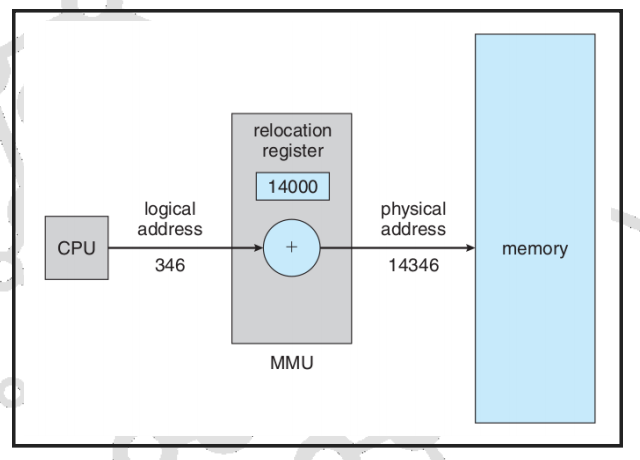
\includegraphics[scale=0.5]{relocation.png}
offset

\vspace{5mm}

\textbf{describe dynamic loading and dynamic linking} \\
\hspace{10mm}dynamic loading is when we load the libraries after load time\\
\hspace{10mm}dynamic linking is when we set the offset after the program have been loaded \\ 
\vspace{5mm}

\textbf{describe swapping and the back stores role} \\
\hspace{10mm} Swapping is when you store memory pages on cold storage due to low/no remaining memory (extremely slow)\\
\hspace{10mm} back stores role \\


\vspace{5mm}
\textbf{describe some algorithm for the dynamic storage-allocation problem} \\
\hspace{10mm} First Fit \\
\hspace{10mm} Worst Fit \\
\hspace{10mm} Best Fit \\

\vspace{5mm}
\textbf{difference between external and internal fragmentation}\\
\hspace{10mm} Internal fragmentation is when there is unused memory within a process allocation \\
\hspace{10mm} external is when there is unused memory between two processes \\

\vspace{5mm}
\textbf{describe segmentation and paging.}\\
\hspace{10mm} segmentation is when you segmentation a program into data, execution code, etc  \\
\hspace{10mm} paging is when you split a program into pages, so there is no external fragmentation, but only internal on the last page of the program.\\








\section{Question 7 - Virtual memory - ch 9}
\subsection{notes}


\subsubsection{Introduction}

\subsubsection{Virtual address space}

\subsubsection{Demand pages}
Means we wont have to load all pages into memory, so processes can start faster. this uses a 

\subsubsection{page fault}
Reference to a page that is not in memory, when this happens the OS check is if valid or not, if its not valid the os will throw an exception, and if its valid the page is loaded into memory, while this is happening the processes is put in a hold state(its a trap) and continued when the page is loaded into memory 
\subsubsection{hardware demand}
page table with valid/invalid\\

\subsubsection{performance of demand paging}

\subsubsection{Page replacement}
\hspace{10mm} first in first out\\
\hspace{10mm} Least recently used\\
\hspace{15mm} can use system clock or a stack with dual pointers, and move it to the top if its used. and always picks the one in button if its used.\\
\hspace{15mm} Needs special hardware, its still slow, due to pointers needing to being changed \\
\hspace{10mm} Second chance \\
\hspace{15mm} clock, first in first out, with a reference bit \\

\hspace{10mm} Least frequently used\\

\hspace{10mm} Most frequently used\\

\hspace{10mm} Optimal page replacement \\
\hspace{15mm}Doesn't exist as we do not know the future. \\
\hspace{15mm}But its good for comparing with other to see how they compare to the optimal.\\

\subsubsection{Page allocation}

\hspace{10mm} Fixed allocation \\

\hspace{15mm} equal allocation \\
\hspace{20mm} dynamic, allocates based on size \\

\hspace{10mm} priority allocation \\

\hspace{15mm} shift memory from low priority to high priority, \\

\subsubsection{Working set}


\newpage
\subsection{Questions from lecture}

Describe demand paging \\
 \hspace{10mm}Bring pages into memory when it is needed, meaning less I/O, less memory needed and faster response. \\

Describe copy on write\\
\hspace{10mm}"Everyone" has a single shared copy of the same data until it's written, and then a copy is made \\

\hspace{10mm}We fork the file so both the parent and the child are using the same file. when a write happen we copy the file so the thread that child and parent aren't working on the same file \\

needs rewriting.\\

Describe the page replacement algorithms\\

\hspace{10mm}FIFO\\
\hspace{15mm}First in first out. removed the oldest page in the buffer if requested one isn't there \& and its out of space.\\
\vspace{5mm}




\hspace{10mm}LRU \\
\hspace{15mm}Least recently used. \\
\hspace{15mm}Uses past knowledge.\\ 
\hspace{15mm}Replaces page that has not been used in the most amount of time \\
\hspace{15mm}Associate time of last use with each page\\
\vspace{5mm}




\hspace{10mm}Counter implementation.\\
 \hspace{15mm}   every page has a counter. \\
\vspace{5mm}





\hspace{10mm}stack implementation  \\
\hspace{15mm}    double link form. \\
    \vspace{5mm}
    
    
\hspace{10mm}Clock \\
\hspace{15mm}circular clock  \\
\vspace{5mm}


\hspace{10mm}LFU \\
\hspace{15mm}Least Frequently Used \\
\hspace{15mm}replaces page with smallest count \\
\hspace{15mm}Can give problems with some pages with lots of use gets "stuck" in the buffer. \\
\vspace{5mm}




\hspace{10mm}MFU \\
\hspace{15mm}based on the argument that the page with the smallest count was probably just brought in and has yet to be used \\
\vspace{5mm}



\hspace{10mm}Optimal \\
 \hspace{15mm}   Impossible as we don't know the future. \\
\vspace{5mm}



What is Beladys Anonmaly \\
\hspace{10mm}Adding more frames can cause more page faults! \\
\vspace{5mm}



Describe trashing \\
\hspace{10mm}If a process does not have enough pages, it gets a lot of page faults causing a lot of pages to be swapped out, only to be swapped in again. \\
\vspace{5mm}


Describe the working-set model. \\
\hspace{10mm}The working set model, tries to predict how many frames we need to allocate for a process. at any given time, (it's dynamic) \\



\vspace{5mm}
Explain buddy system \\
\hspace{15mm}Allocate memory from a fixed size segment. \\


\subsection{Keywords}

1. **Introduction / Benefits**  \\
		- Why do we need this? \\
		- The relationship between virtual and physical memory. \\

\vspace{5mm}

2) **Demand paging**  \\
		- Concepts, Page-replacement algorithms, Page-faults \\
		- Performance of demand paging. \\

\vspace{5mm}

3) **Copy-on-Write**  \\
		- General idea: why keep identical copies of pages in memory? \\

\vspace{5mm}

4) **Page replacement**  \\
\hspace{10mm} - If we run out of memory, which pages should we replace?) \\


\hspace{10mm}FIFO\\
\hspace{15mm}First in first out. removed the oldest page in the buffer if requested one isn't there \& and its out of space.\\
\vspace{5mm}




\hspace{10mm}LRU \\
\hspace{15mm}Least recently used. \\
\hspace{15mm}Uses past knowledge.\\ 
\hspace{15mm}Replaces page that has not been used in the most amount of time \\
\hspace{15mm}Associate time of last use with each page\\
\vspace{5mm}




\hspace{10mm}Counter implementation.\\
 \hspace{15mm}   every page has a counter. \\
\vspace{5mm}



\hspace{10mm}stack implementation  \\
\hspace{15mm}    double link form. \\
    \vspace{5mm}
    
    
\hspace{10mm}Clock \\
\hspace{15mm}circular clock  \\
\vspace{5mm}


\hspace{10mm}LFU \\
\hspace{15mm}Least Frequently Used \\
\hspace{15mm}replaces page with smallest count \\
\hspace{15mm}Can give problems with some pages with lots of use gets "stuck" in the buffer. \\
\vspace{5mm}




\hspace{10mm}MFU \\
\hspace{15mm}based on the argument that the page with the smallest count was probably just brought in and has yet to be used \\
\vspace{5mm}



\hspace{10mm}Optimal \\
 \hspace{15mm}   Impossible as we don't know the future. \\
\vspace{5mm}

\vspace{5mm}

5) **Allocation of frames**  \\
		- Which process get n number of frames \\

\vspace{5mm}

6) **Thrashing** \\
		- Page-replacement gone wild, pdf p450 \\

\vspace{5mm}

7) **Memory-Mapped Files**  \\
		- Hard to read\\












\section{Question 8 - file system \& Implementing filesystems - ch 10 and 11}

May ask things about process control block


\subsection{Notes}
\subsubsection{objectives}

Explain the function and interfaces of file systems\\

Discuss file-system design tradeoffs, including access
methods, file sharing, file locking, and directory structures
Explore file-system protection \\

Describe the details of implementing local file systems
and directory structures\\


Describe the implementation of remote file systems \\

Discuss block allocation and free-block algorithms and
trade-offs
\\



\subsubsection{File control block}
File permissions

File dates (created, access, edited)

add more



\subsubsection{Questions from lecture}

Describe different directory structures and their implementations 
	single level
		One directory for all users
		
	two level
		one Directory or each user
	tree structure
		infinite number of directories
	General graph
		Link only to files.
	ACYCLIC-GRAPH
		Link

Describe protection measures in file systems

	Creator can set perms on a file.	
	
	Access control list
		Read
		Write,
		Execute
		Append
		Delete
		List
		
	

Describe the layers in a file system

	Application programs.
		Doesnt care about anything
	logical file system.
		Cares about user rights
	file-organization module.
		
	Basic file system.
	I/O control.
		Knows how to talk with the different devices.
	devices.


What does a device driver do?
	
	Translator from file id, to sector on drive.

What does a FCB contain
	
	File permissions
	Size
	Owner, group, ACL(Access control list)
	File dates, created, acess, edited
	File data blocks, or pointers to data blocks (INode)

Describe different methods for locating data for a file
	
	INDEXED ALLOCATION

	LINKED SCHEME
	
	MULTILEVEL INDEX
	
	COMBINED SCHEME\\
	

Describe methods for free space management

	Free list
		Linked list
		

	




\subsection{Keywords}
Intro\\
	i-node\\
	
	
\vspace{5mm}
	
	
Files\\
\hspace{10mm}	Files operations\\
\hspace{10mm}	How you read the files. linked, segmented, random.\\
	
	
\vspace{5mm}
	
	
Directories\\
\hspace{10mm}	How do we know what files and subdirectories are in the directory.\\
	
	
	
\vspace{5mm}
	
Disk structure\\


\vspace{5mm}
File system mounting \\


\vspace{5mm}
File sharing \\

\vspace{5mm}
File access(Protection/permissions)\\
\hspace{10mm} Owner groups\\

\vspace{5mm}
Recovery \\


\vspace{5mm}
Network files \\



\vspace{5mm}
Allocation \\


\vspace{5mm}
Free Space management \\

\hspace{10mm}



	




\section{Question 9 -Mass-Storage Structure and I/O Systems - ch 12 and 13 }

\subsection{notes}
\subsubsection{Disk}
1-dimensional array of logical blocks\\

Sector 0 is the first sector on the outermost track \\

\subsubsection{Disk - Scheduling}
SSTF
Shortest seek time first.
may cause starvation\\

Scan
Go from lowest index, to highest, and back to lowest, also known as elevator algor.\\



C-scan
Go from lowest index, to highest, and back to lowest without reading.\\



look
Go from lowest index in queue, to highest in queue, and back to lowest in queue without reading.\\
\subsubsection{Disk - Sector}
Header information, Data, ecc code \\






\subsection{Questions from lecture}
	What are the similarities and differences between NAS and SAN \\
		\textcolor{red}{TODO}
	Describe the disc scheduling algorithms; \\
		FCFS, \\
		First come first serve\\
		
		SSTF, \\
		Shortest search first \\
			
		SCAN, \\
		all the way from first sector to last sector and back.\\
		
		LOOK \\
		Like scan by only goes from element to element, and doesn't start from the beginning. \\	
	
		C-Scan, \\
		like scan but doesn't read on the way back \\
		
		
		C-look		
		Like scan  but doesn't read on the way back
		
	Describe sector sparing
		If the drive encounter a sector it can't write to it will then jump and write to a different sector that it has already allocated.
	
	Describe raid and the mechanisms used
	raid 0
		split the data on multiple disks for more speed
	raid 1
	
		copy the data on multiple disk if one fails you wont loose the data.
	raid 2 (Bits striped)
	
	two groups of disk, one group is data, one disk stores the correction code.
	raid 3(bytes striped)
	
		dedicated storage disks and a dedicated parity disk
		
	raid 4(blocks Striped)
	same just with blocks
	
	raid 5(blocks striped, and distributed parities)
	
	raid 6(blocks striped, and two distributed parities)
	
	
	raid 10
	
	What is stable storage and how can yo achieve it
	
	Name some of the characteristics of i/o devices
	
	Explain caching, spooling and device reservation
	

\subsection{Keywords}
Introduction
\hspace{10mm} \textbf{Ex} \\

Disk Scheduling 
\hspace{15mm} \textbf{FCFS} \\
\hspace{15mm} \textbf{Look} \\
\hspace{15mm} \textbf{SSFT} \\
\hspace{15mm} \textbf{FCFS} \\



Disk manegment 
\hspace{5mm} \textbf{•} \\


Raid (read) http://igoro.com/archive/how-raid-6-dual-parity-calculation-works/
\hspace{5mm} \textbf{Raid 5/6} \\
\hspace{5mm}	raid 0
\hspace{10mm}		split the data on multiple disks for more speed
\hspace{5mm}	raid 1
	
\hspace{10mm}		copy the data on multiple disk if one fails you wont loose the data.
\hspace{5mm}	raid 2 (Bits striped)
	
\hspace{10mm}	two groups of disk, one group is data, one disk stores the correction code.
\hspace{5mm}	raid 3(bytes striped)
	
\hspace{10mm}		dedicated storage disks and a dedicated parity disk
		
\hspace{5mm}	raid 4(blocks Striped)
\hspace{10mm}	same just with blocks
	
\hspace{5mm}	raid 5(blocks striped, and distributed parities)
	
\hspace{5mm}	raid 6(blocks striped, and two distributed parities)
\hspace{10mm}	Parity is often calculated but xoring the data and saving the output as a parity.
	
	raid 10
I/O devices
	buses, and controllers and port
 
I/O Hardware
	How do to I/O talk to hardware
	Busy bit where the host waits until the devices is ready.
	Interrupts blocks the I/O devices
	Direct memory access.

I/O Streams
	

\section{Question 10 - System Protection - ch 14}



\subsection{Keywords}

Introduction \\
Domains \\
	access matrix \\
Revocation of access rights.\\
capability based system\\
	Need to know \\
Language based protection\\
Types of attacks \\



\subsection{Questions from lecture}

Describe how an access matrix is used and what it contains \\


How can you implement the access matrix \\

What security measure levels should you handle\\

Describe the principles in the following attacks: stack and buffer overflow, virus, trap door.\\

Describe differences between symmetric and asymmetric cryptology\\

What is an authenticator\\


\section{Question 11 - System Security - ch15}



\subsection{Keywords}

Introduction \\
Types of attack \\
	Trojan horse \\
	logic bomb \\

symmetrical and asymmetrical encryption \\
	1 key vs 2 key\\
	b64 vs rsa \\
	RSA \\

User authentication \\
	How to store passwords(not everyone should have access). \\
	Firewalls \\
	

\subsection{Questions from lecture}

\section{Question 12 - Virtual Machines cp-16 }



\subsection{Keywords}
1) **Introduction** 
		What is it.
			Containers, 
		
		Why should we use it?
		Security
		(Explain what virtualization is, and what a virtual machine is. The figure from above is good. )
		
		
2) **History** 
		(This should go with the introduction if mentioned)
		
		
		
3) **Benefits and Features** 
	Security
		Safer as machines are isolated from each other.
	Testing software in an isolated environment.
	live Migration We can move machines to other hardware without stopping them.
		
	Snapshots
	
	there's a tiny bit of performance overhead.
		
		
4) **Building Blocks** 
		(Very important - explains how it works, two method especially: Trap-and-Emulate/Binary translation, See p717)
		
		Trap and emulate , block systems calls and emulated what they did.
		Binary translation, translates it to something that doesn't cause it to damage the host, or if the hardware doesn't support the function.
		
		
		
		
5) **Types of Virtual Machines and Their Implementations** 
		Type 0 hyper visor - Hardware based.
		Type 1 Hypervisor  - Specific vm based os vmware(window uses this for hyper-v)
		type 2 Hypervisor  - Normal os with a vm container program
		
		Paravirtualization 
		
		
6) **Virtualization and Operating-System Components** 
		Nested page tables.
		(Extends (4) and goes into details of how many of the concepts we learned, are transferred into the virtual system.)


\subsection{Questions from lecture}
Describe the role of the VMM/hypervisor:\\
	The mange the virtual machines, hardware access, and port forwarding, and such, may only do virtual switches, and more.\\

	


What is an emulator\\
	Program that emulates a different operating system or set of hardware.\\


Name some of the benefits of virtualisation\\
	the processes are separated within the same hardware, and you can run multiple different different operating systems on the same hardware.\\
		Snapshots\\
	use hardware more efficiently\\
	Live migration\\


Describe the "trap and emulate" and "binary translation"\\
	We don't want the user to access the kernel mode on the hardware.\\
	
	So the VMM does all the kernal operations, its just very expensive.\\

Why are nested page tables used\\
	Because each VM has its own memory.\\
		

How is live-migration preformed\\
	1. create new vm on new host\\
	2. move read only pages to new host\\
	3. move read/write pages to new host\\
	4. move dirty pages to new host, and check if there are changes to read/write pages and move those.\\
	5. pause the vm, move the last pages, and point network traffic to new host. \\
	6. shut down old vm. \\


\section{Question 13 -  Networks and Distributed Systems  cp-17 }



\subsection{Keywords}
1) **Introduction** 
	- Advantages of Distributed Systems, such as Resource sharing/Speedup/Reliability. 
	- Disadvantages would be a nice touch too.
2) **Types of Network-based Operating Systems** 
	- Network OS/Distributed OS
	- What are the differences?
3) **Network Structure** 
	- LAN and WAN, also known as Local Area Network and Wide Area Network, difference being how they are physically placed 
	- WAN is the network between the different campus' here at SDU
4) **Communication Structure** 
	- The gritty details of how the CPUs communicate, very important. 
	- Especially stuff such as routing strategies.
5) **Communication Protocols** 
	- Same as above
6) **Robustness** 
	- How can we make the system more robust regarding system failure, or network failure
7) **Design Issues** 
	- What are some typical design issues that needs to be handled, 
	**notice how this section could let many here learn what a typical design section might be**
8) **Distributed File Systems** 
	- OpenAFS, NFS
9) **Examples** 
	Book offers several examples, mentioning these can often be a nice touch, when explaining the rest.
	



\end{document}
